\documentclass{standalone}
\usepackage{tikz}
\usetikzlibrary{decorations.pathmorphing} % For wavy lines

% Define a style for wavy lines
\tikzset{
    wavy/.style={
        decorate,
        decoration={snake, amplitude=.4mm, segment length=2mm, post length=0mm}
    }
}

\begin{document}
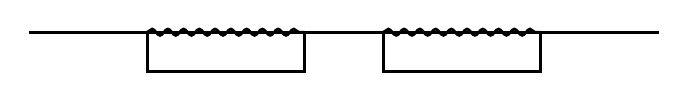
\begin{tikzpicture}[line width=1pt]

% Draw the horizontal straight lines
\draw (0,0) -- (8,0);

% Draw the first twist region (saddle move)
\draw[wavy] (1.5,0) -- (3.5,0);
\draw (1.5,0) -- (1.5,-0.5) -- (3.5,-0.5) -- (3.5,0);

% Draw the second twist region (saddle move)
\draw[wavy] (4.5,0) -- (6.5,0);
\draw (4.5,0) -- (4.5,-0.5) -- (6.5,-0.5) -- (6.5,0);

% Add some annotations if needed (optional)
% \node at (0.5,0.2) {$\varphi$};

\end{tikzpicture}
\end{document}